\section{Les écrans de l'application}
\label{sec:pages-presentation}

La sous-section \ref{subsec:requested-pages} établissait une série de pages nécessaires que je vous propose de découvrir ici.
La barre de navigation est présente sur toutes les pages mais je l'ai omise dans la plupart des cas pour gagner de la place et éviter la redondance.

\begin{figure}[ht]
    \centering
    
\includegraphics[width=1\textwidth]{images/screenshot/navbar-visitor.png}
    \caption{La barre de navigation vu par le \textbf{visiteur}, s'il désire naviguer vers la validation, l'application lui ouvrira le menu pour se connecter}
    \label{fig:navbar-visitor}
\end{figure}

\begin{figure}[ht]
    \centering
    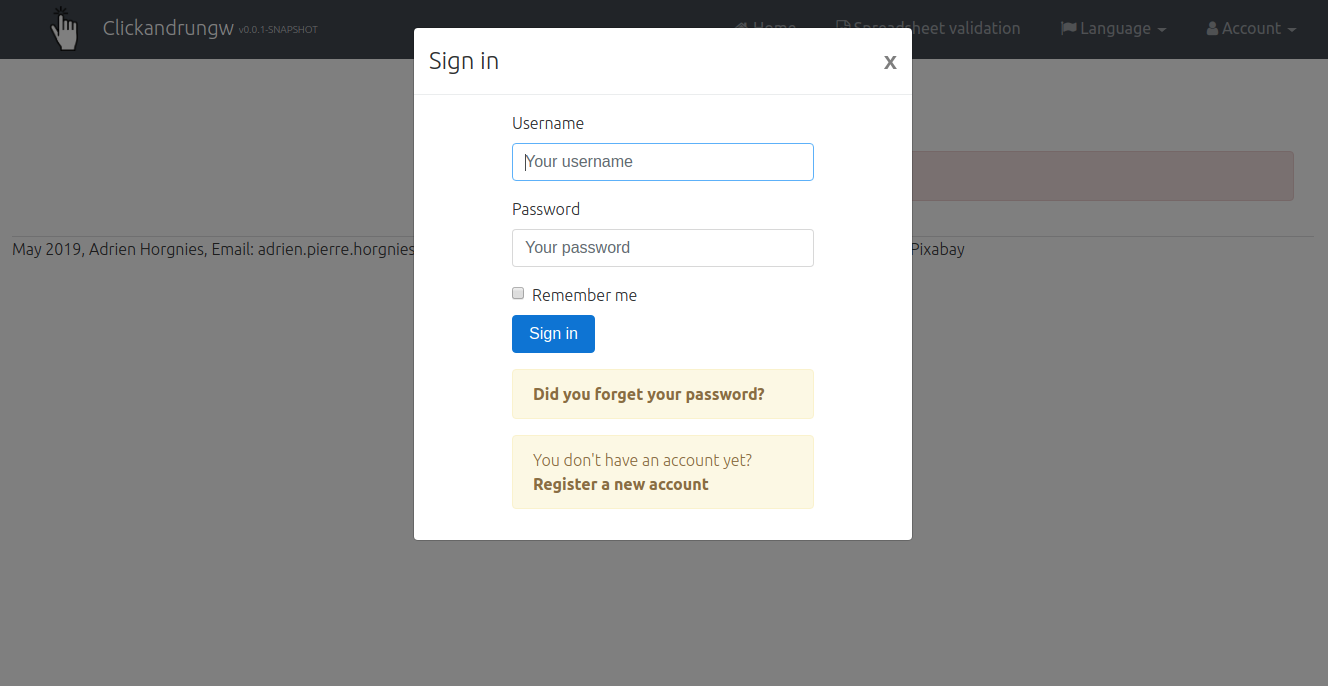
\includegraphics[width=1\textwidth]{images/screenshot/login-modal.png}
    \caption{La modale qui s'ouvre par-dessus la page pour demande à l'utilisateur de se connecter}
    \label{fig:login-modal}
\end{figure}

\begin{figure}[ht]
    \centering
    
\includegraphics[width=1\textwidth]{images/screenshot/navbar-user.png}
    \caption{La barre de navigation vue par l'\textbf{utilisateur}}
    \label{fig:navbar-user}
\end{figure}

\begin{figure}[ht]
    \centering
    
\includegraphics[width=1\textwidth]{images/screenshot/navbar-admin.png}
    \caption{La barre de navigation vue par l'\textbf{administrateur}}
    \label{fig:navbar-admin}
\end{figure}

\begin{figure}[ht]
    \centering
    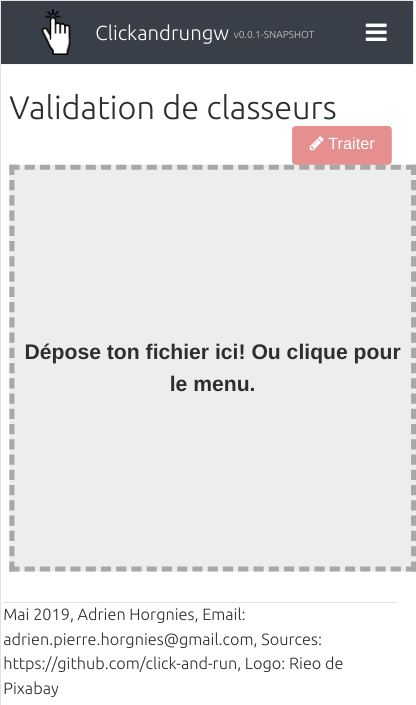
\includegraphics[width=0.4\textwidth]{images/screenshot/navbar-hamburger-closed.png}
    \caption{La barre de navigation fermée sur \textit{smartphone}}
    \label{fig:navbar-hamburger-closed}
\end{figure}

\begin{figure}[ht]
    \centering
    
\includegraphics[width=0.4\textwidth]{images/screenshot/navbar-hamburger-open.png}
    \caption{La barre de navigation ouverte sur \textit{smartphone}}
    \label{fig:navbar-hamburger-opened}
\end{figure}

\begin{figure}[ht]
    \centering
    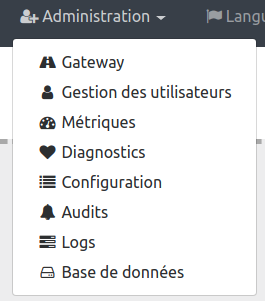
\includegraphics[width=0.4\textwidth]{images/screenshot/menu-admin.png}
    \caption{Le menu des outils d'administration, le menu le plus fourni en éléments}
    \label{fig:menu-admin}
\end{figure}
\paragraph{}

\begin{figure}[ht]
    \centering
    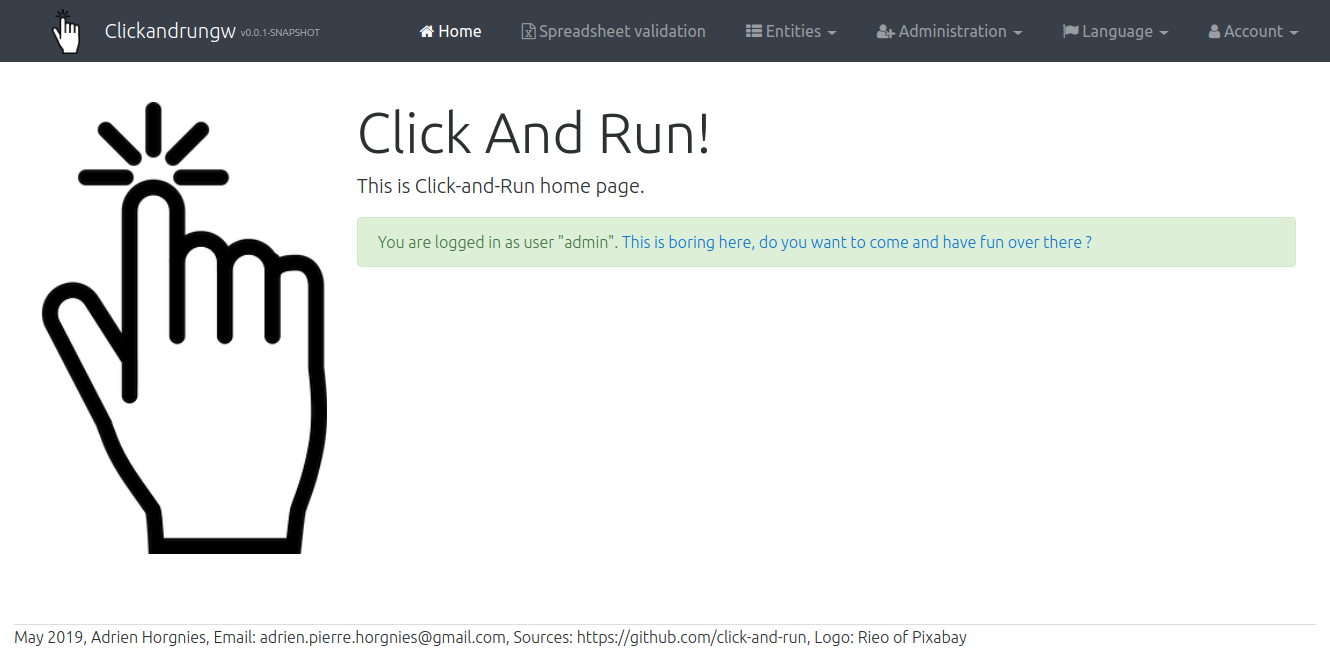
\includegraphics[width=1\textwidth]{images/screenshot/home-page-logged.png}
    \caption{La page d'accueil pour les \textbf{utilisateurs} et l'\textbf{administrateur}}
    \label{fig:home-logged}
\end{figure}

\begin{figure}[ht]
    \centering
    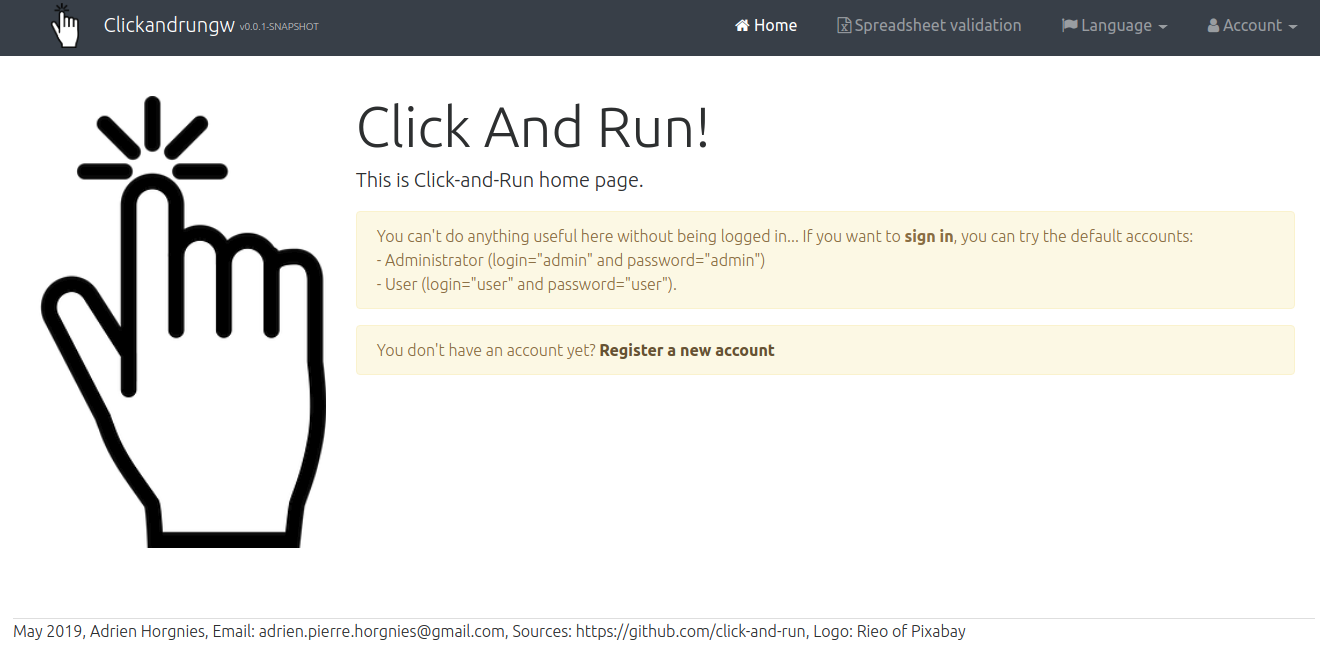
\includegraphics[width=1\textwidth]{images/screenshot/home-page-anon.png}
    \caption{La page d'accueil pour les \textbf{visiteurs}}
    \label{fig:home-anon}
\end{figure}

\begin{figure}[ht]
    \centering
    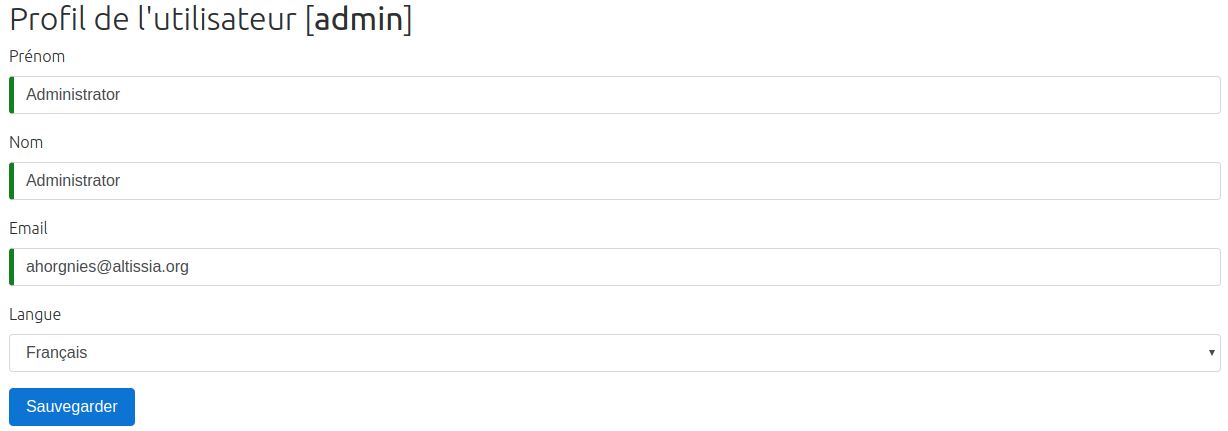
\includegraphics[width=1\textwidth]{images/screenshot/account-profile.png}
    \caption{La page du profil}
    \label{fig:account-profile}
\end{figure}

\begin{figure}[ht]
    \centering
    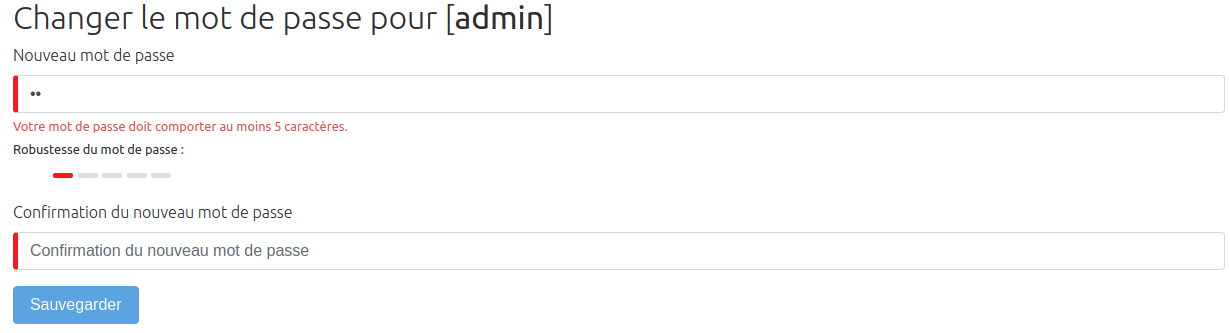
\includegraphics[width=1\textwidth]{images/screenshot/account-password.png}
    \caption{La page du mot de passe}
    \label{fig:account-password}
\end{figure}

\begin{figure}[ht]
    \centering
    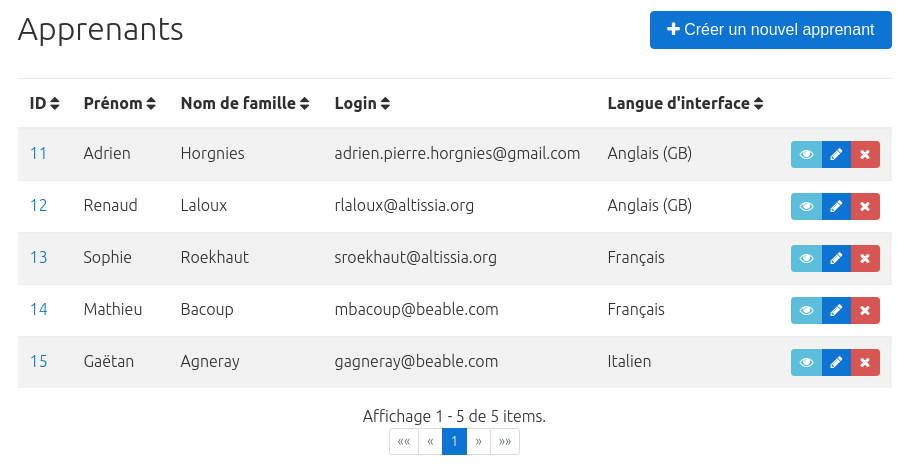
\includegraphics[width=1\textwidth]{images/screenshot/entity-learners.png}
    \caption{La page de l'entité apprenant sur écran de taille réduite}
    \label{fig:entity-learner}
\end{figure}

\begin{figure}[ht]
    \centering
    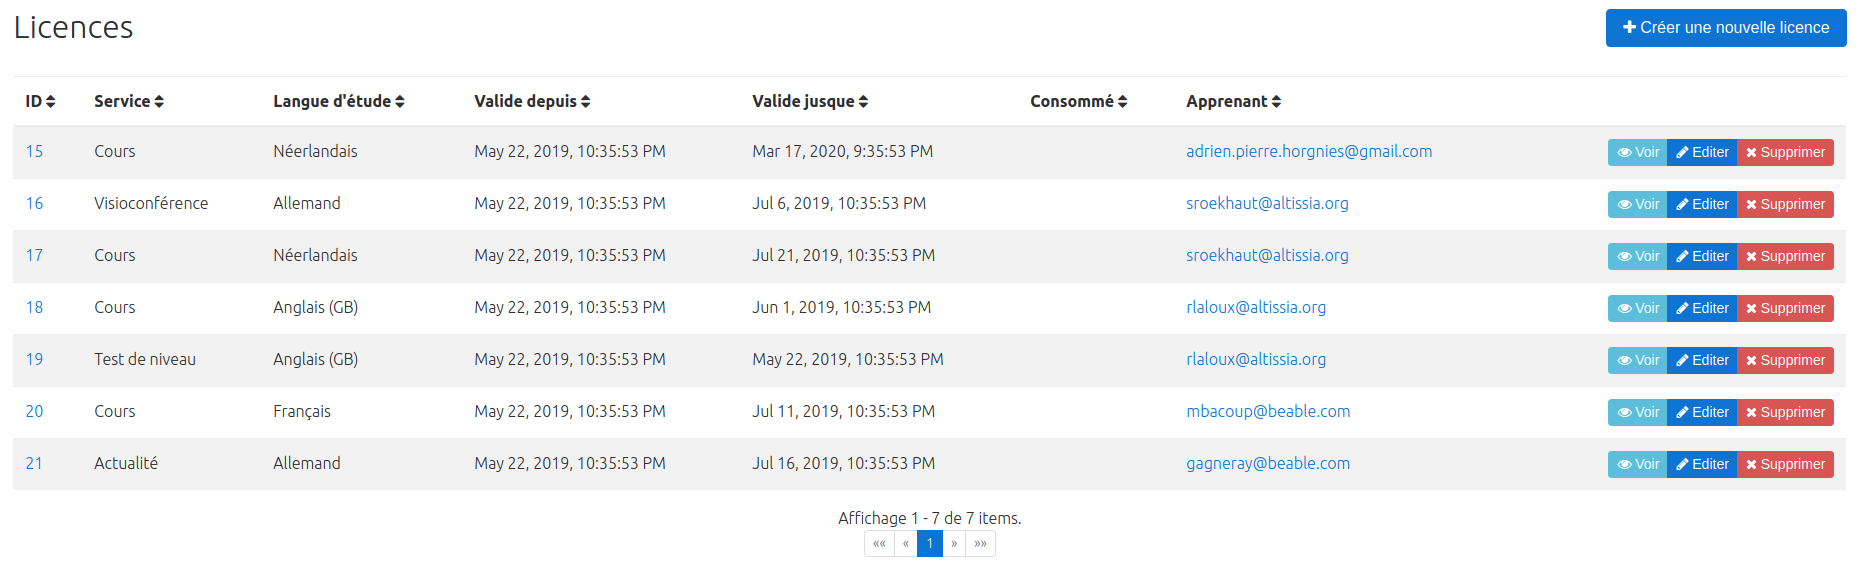
\includegraphics[width=1\textwidth]{images/screenshot/entity-licenses.png}
    \caption{La page de l'entité licence}
    \label{fig:entity-license}
\end{figure}

\begin{figure}[ht]
    \centering
    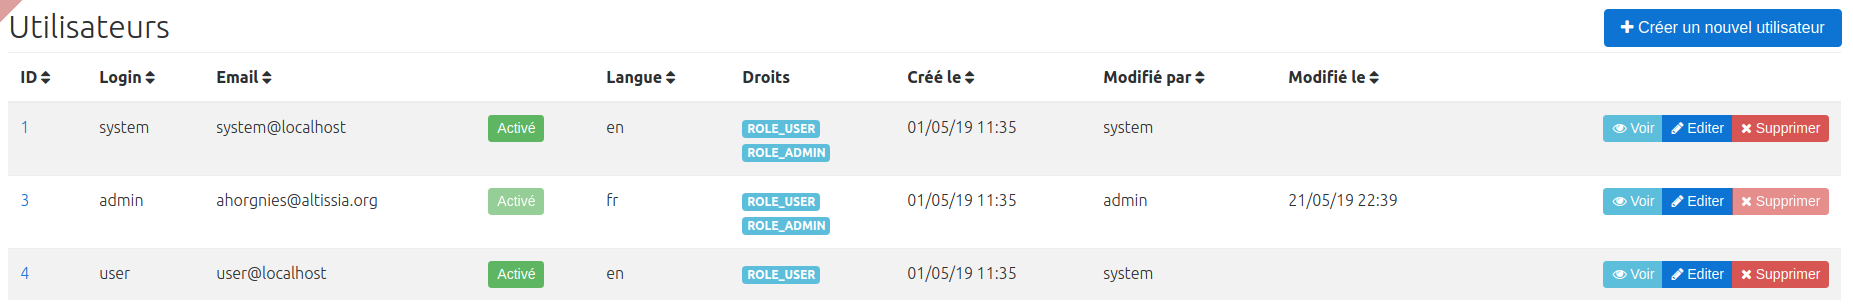
\includegraphics[width=1\textwidth]{images/screenshot/admin-users.png}
    \caption{La page d'administration de gestion des utilisateurs}
\end{figure}

\begin{figure}[ht]
    \centering
    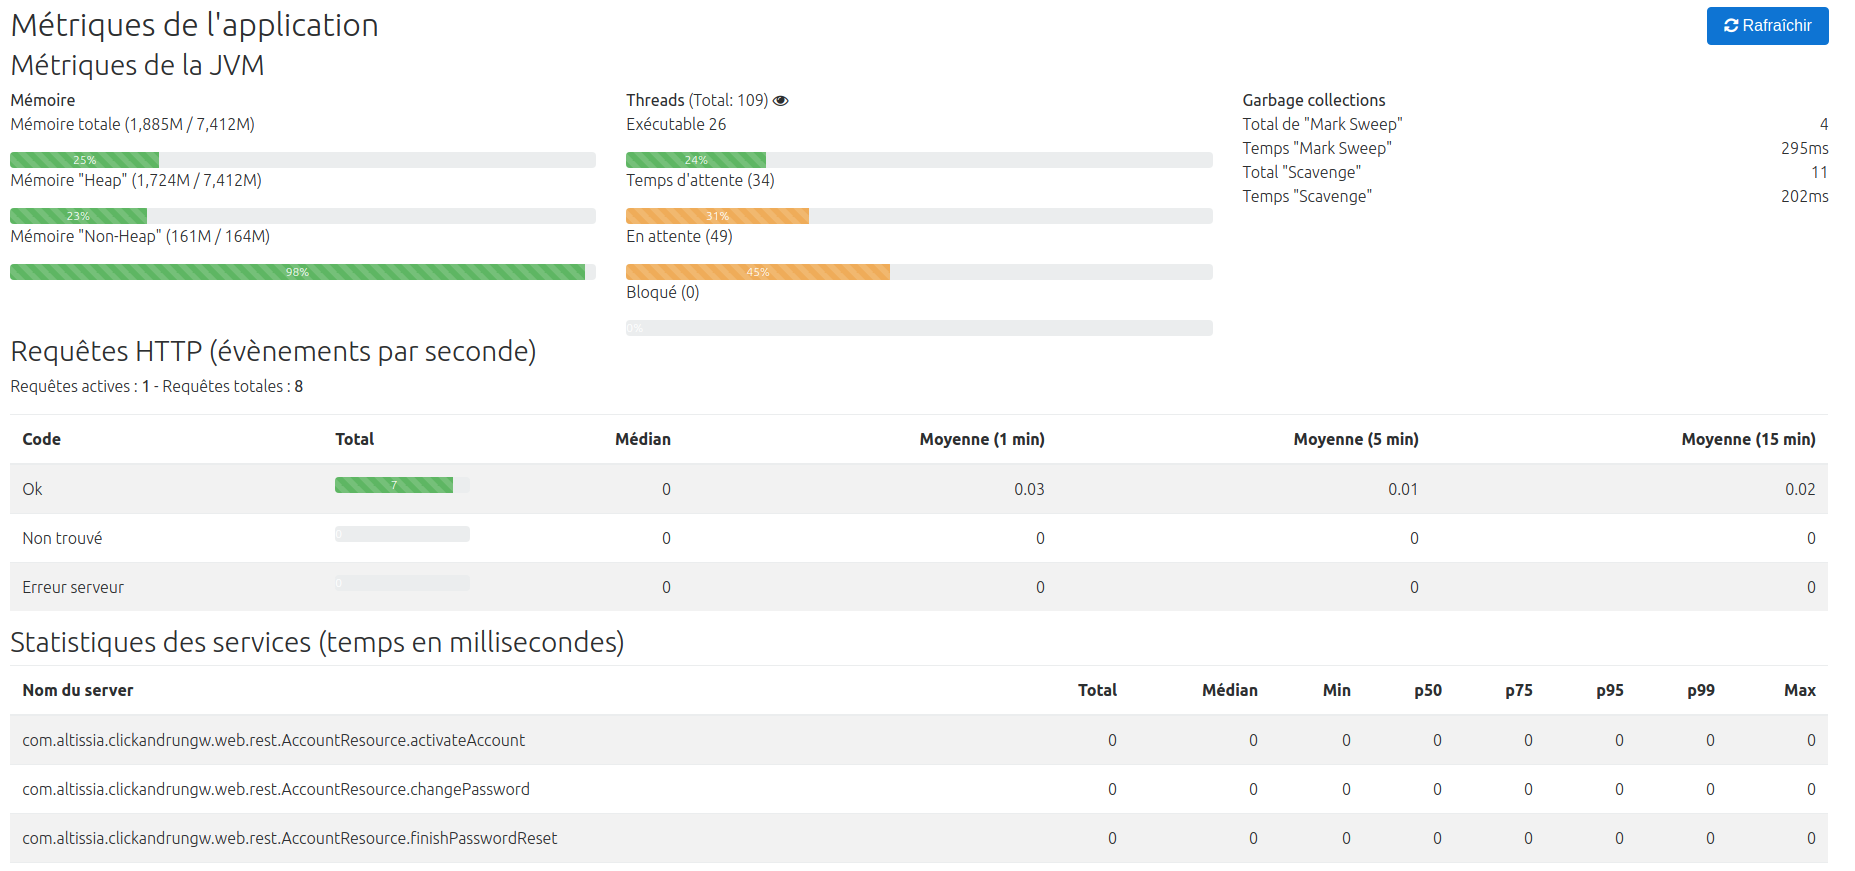
\includegraphics[width=1\textwidth]{images/screenshot/admin-metrics.png}
    \caption{La page d'administration de surveillance du \gls{g-server}}
\end{figure}

\begin{figure}[ht]
    \centering
    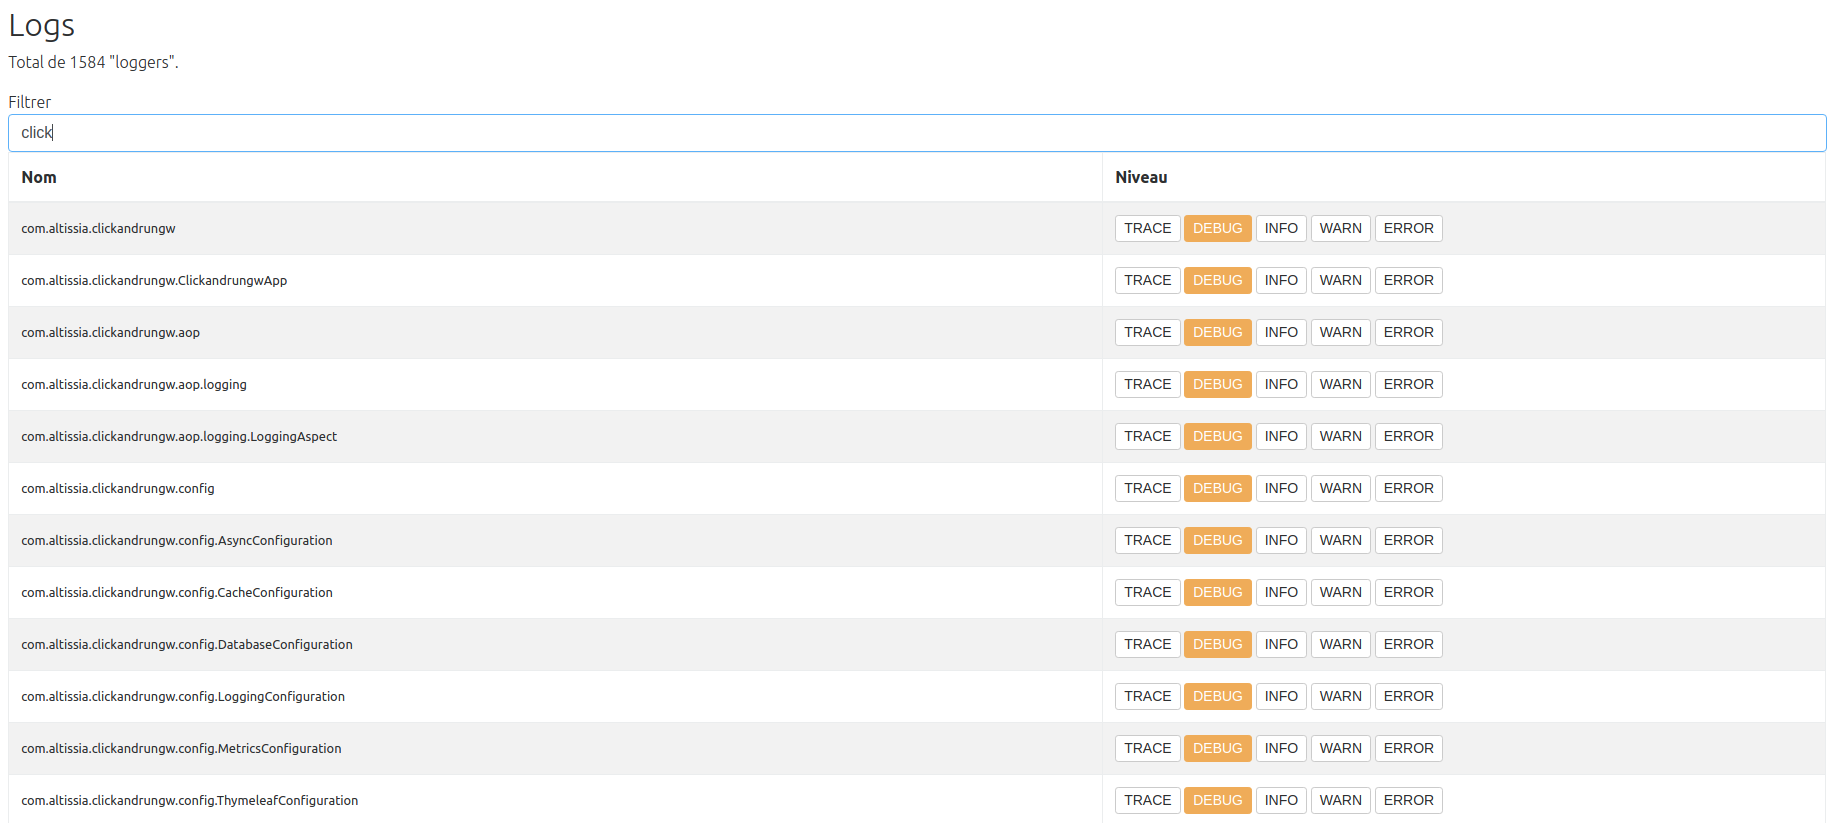
\includegraphics[width=1\textwidth]{images/screenshot/admin-logs.png}
    \caption{La page d'administration de contrôle des niveaux de verbosité des journaux d'application}
\end{figure}

\begin{figure}[ht]
    \centering
    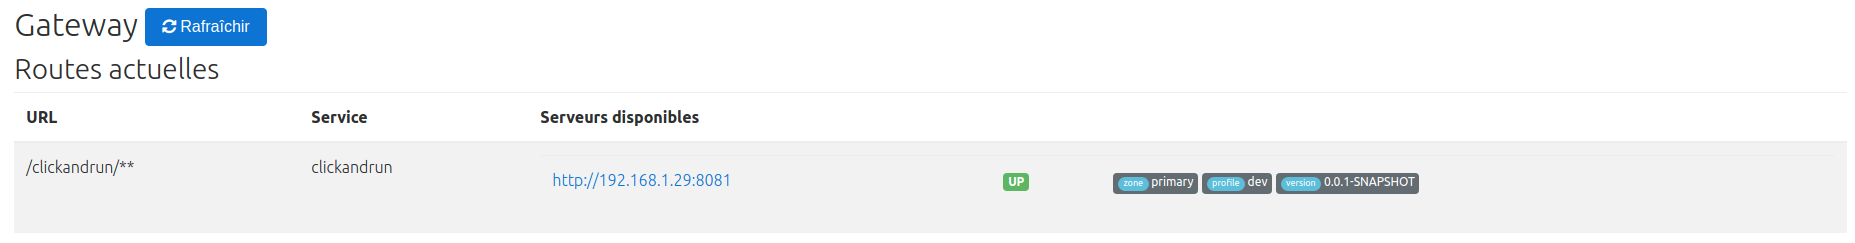
\includegraphics[width=1\textwidth]{images/screenshot/admin-gateway.png}
    \caption{La page d'administration de surveillance des services externes disponibles}
\end{figure}

\begin{figure}[ht]
    \centering
    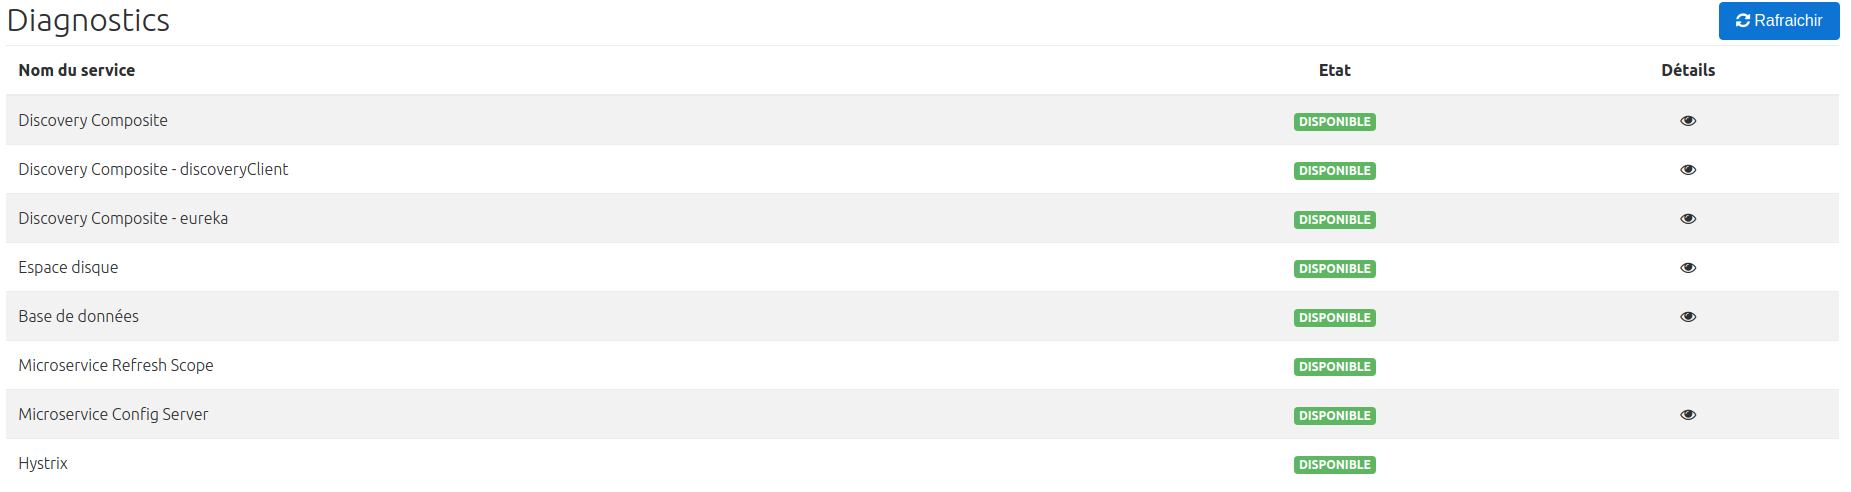
\includegraphics[width=1\textwidth]{images/screenshot/admin-diagnostics.png}
    \caption{La page d'administration de surveillance des services internes disponibles}
\end{figure}

\begin{figure}[ht]
    \centering
    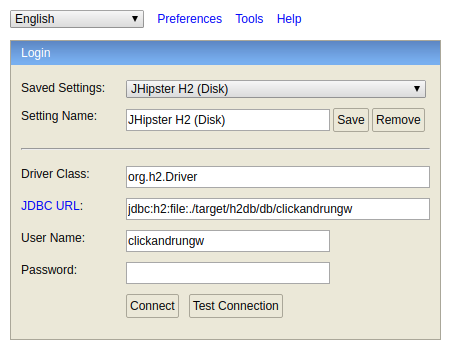
\includegraphics[width=1\textwidth]{images/screenshot/admin-db.png}
    \caption{La page d'administration d'accès à la base de données; elle dépend de l'outil d'administration choisi, ici c'est la console de H2, une base de données de développement}
\end{figure}

\begin{figure}[ht]
    \centering
    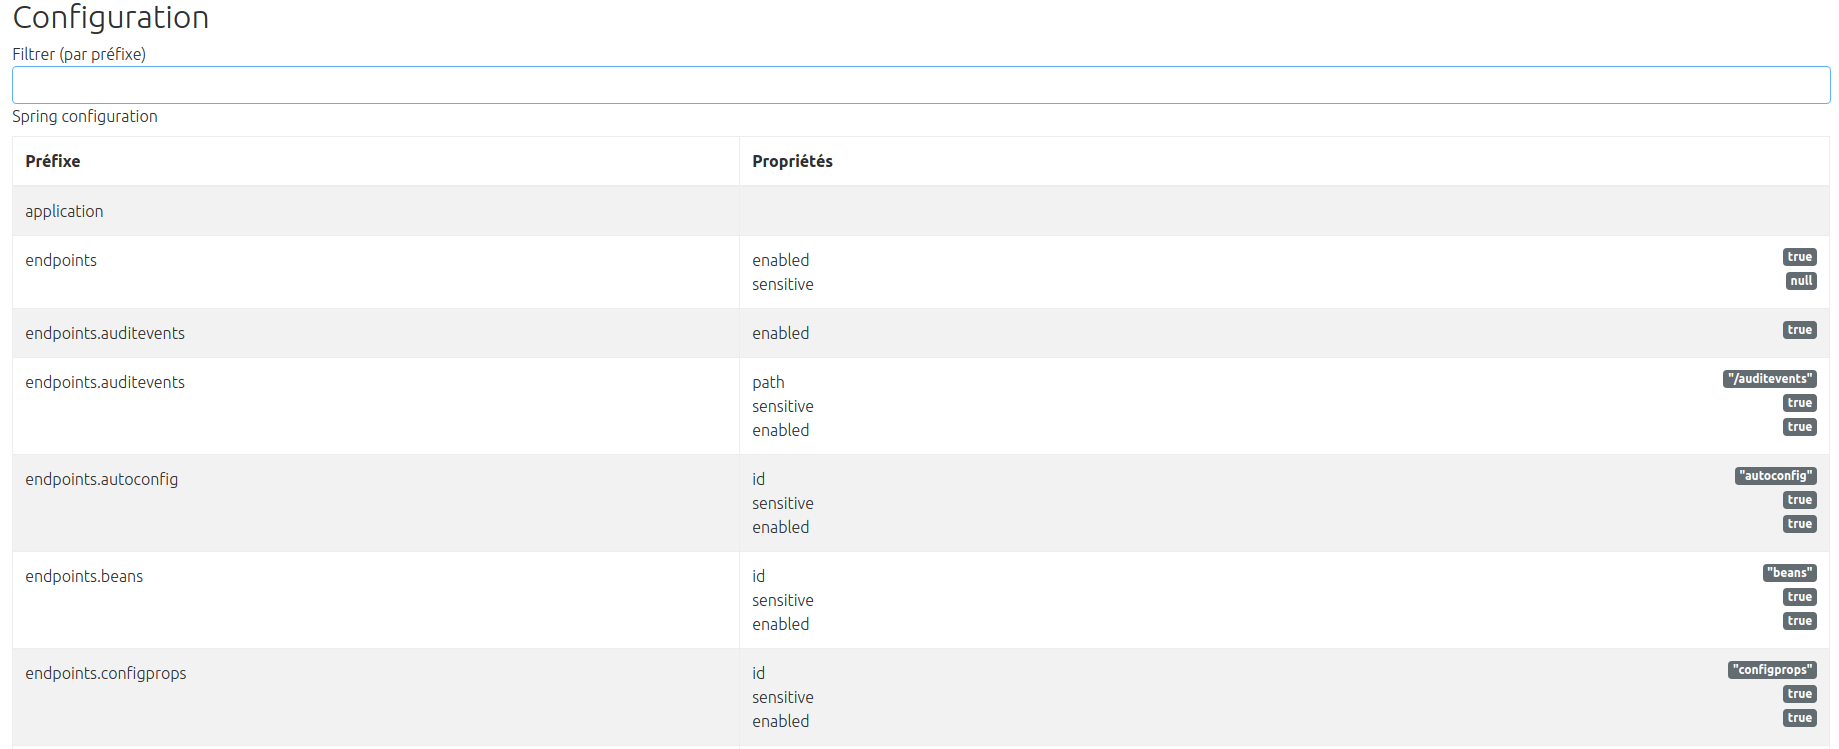
\includegraphics[width=1\textwidth]{images/screenshot/admin-config.png}
    \caption{La page d'administration pour consulter la configuration appliquée}
\end{figure}

\begin{figure}[ht]
    \centering
    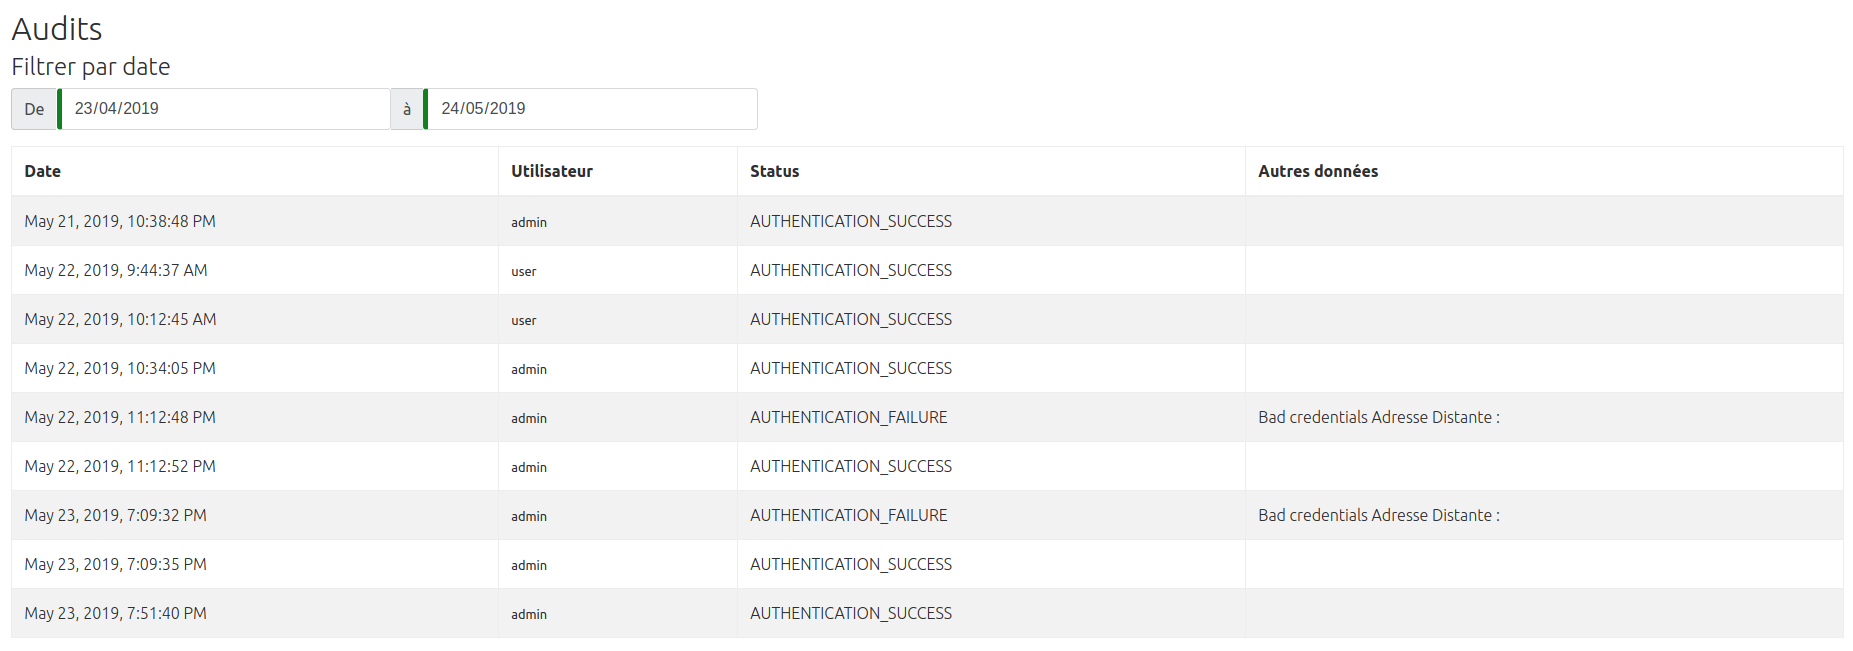
\includegraphics[width=1\textwidth]{images/screenshot/admin-audits.png}
    \caption{La page d'administration de surveillance des évènements audités}
\end{figure}

\begin{figure}[ht]
    \centering
    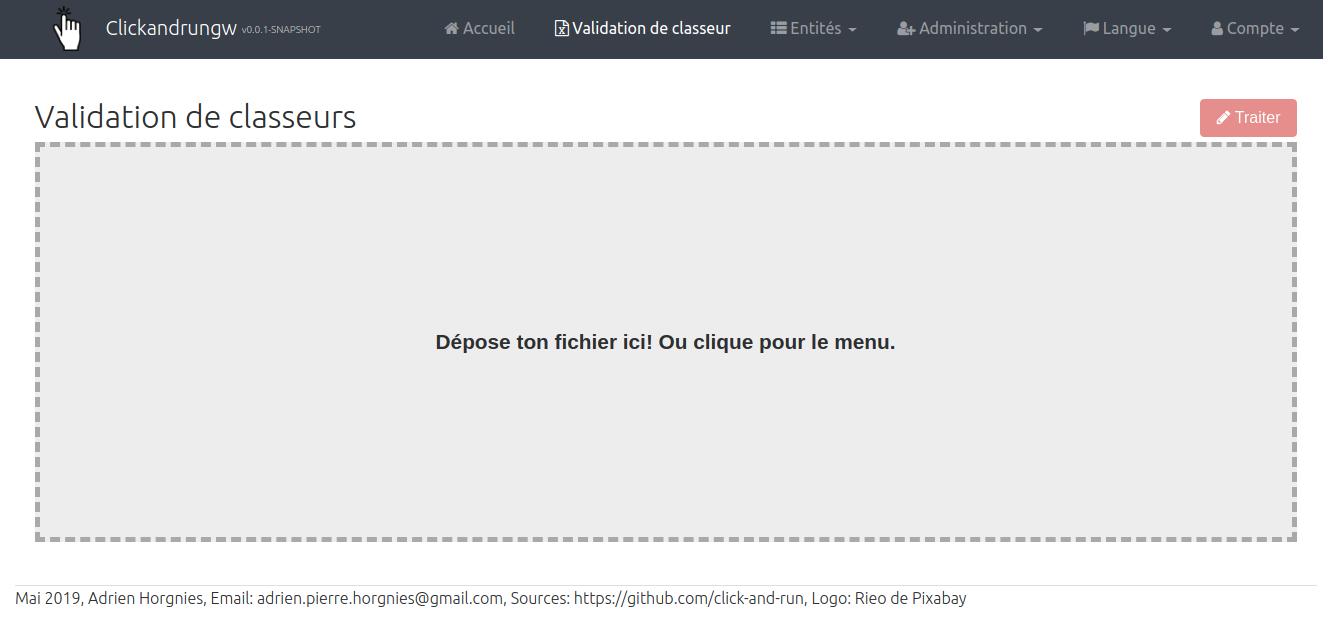
\includegraphics[width=1\textwidth]{images/screenshot/validation-empty.png}
    \caption{La page de validation prête à ếtre utilisée}
\end{figure}

\begin{figure}[ht]
    \centering
    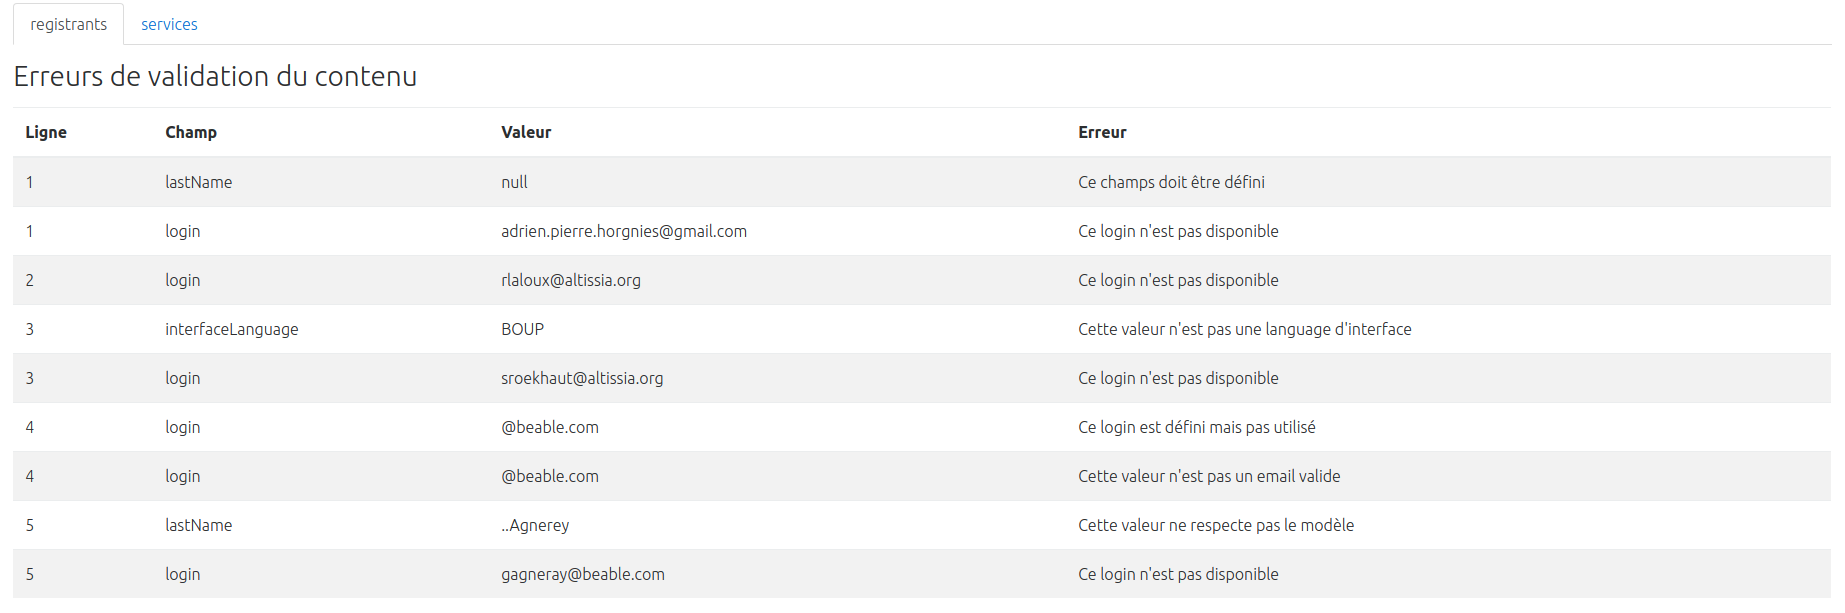
\includegraphics[width=1\textwidth]{images/screenshot/validation-registrants.png}
    \caption{Le dessous de la page de validation présentant des erreurs dans les apprenants}
\end{figure}

\begin{figure}[ht]
    \centering
    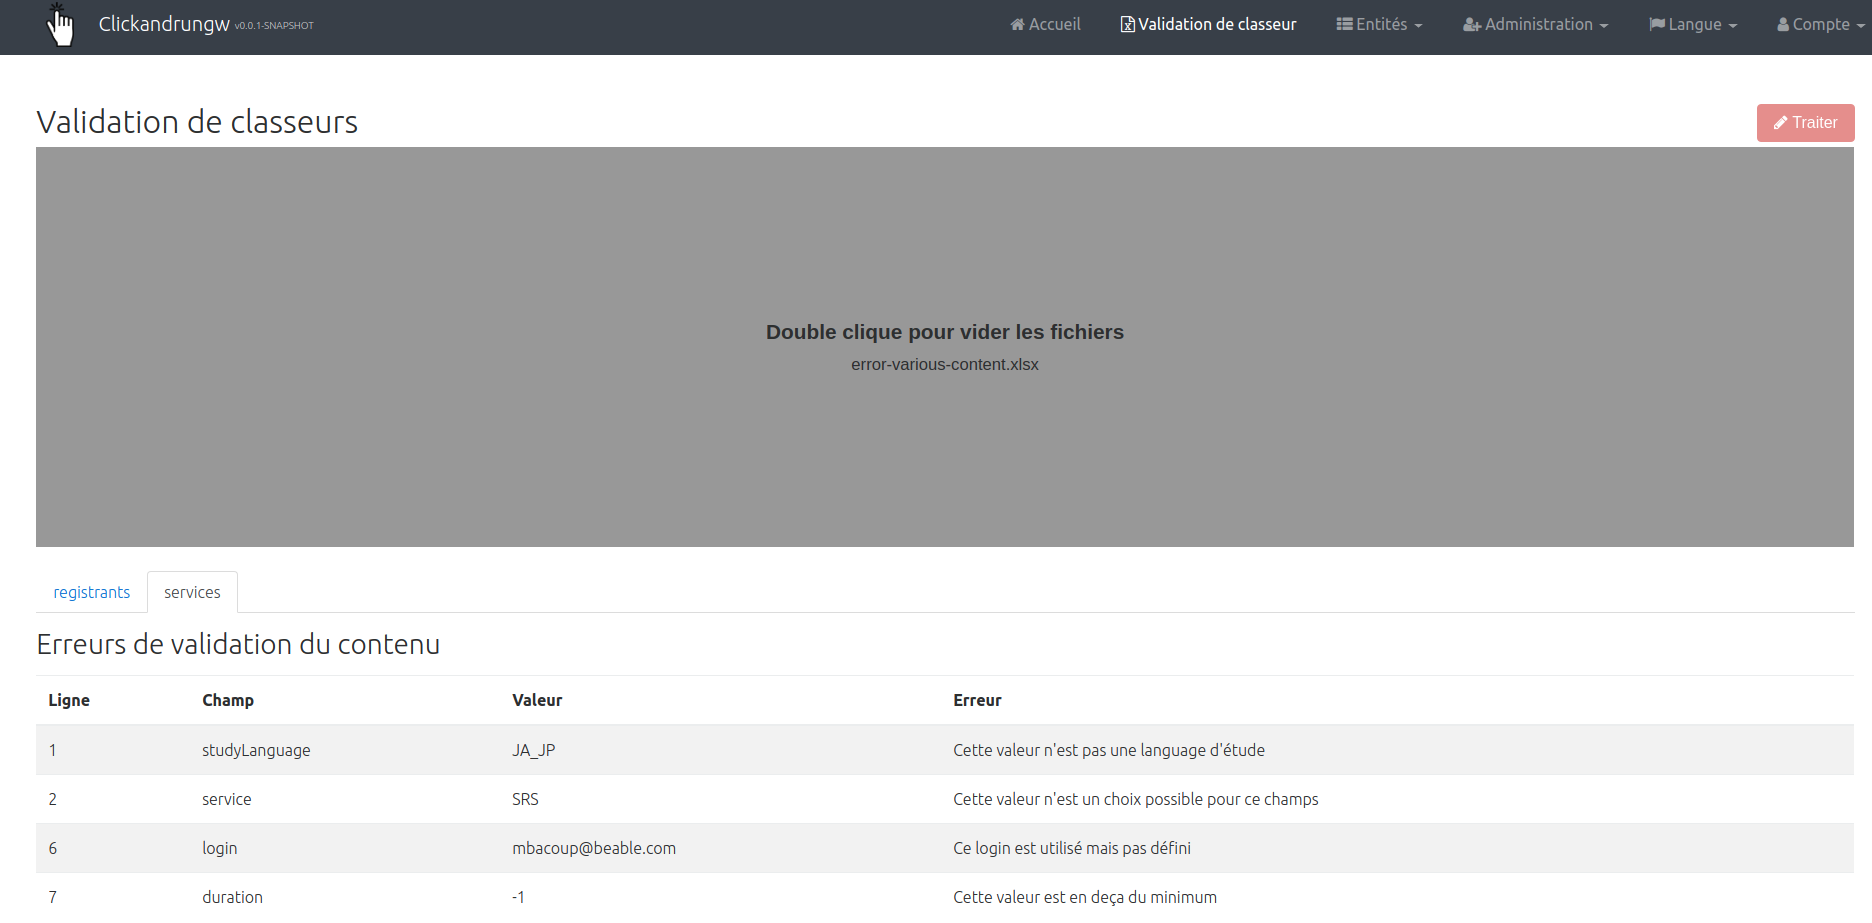
\includegraphics[width=1\textwidth]{images/screenshot/validation-services.png}
    \caption{La page de validation présentant l'onglet des erreurs dans les services}
\end{figure}
